\documentclass[letter]{article}
\usepackage{amsmath, amsthm, amssymb, multicol, enumitem}
\usepackage[margin=0.5in]{geometry}
\usepackage{tikz}

\usepackage{titlesec}

\titlespacing\section{0pt}{4pt plus 2pt minus 2pt}{2pt plus 2pt minus 2pt}
\titlespacing\subsection{0pt}{2pt plus 2pt minus 2pt}{2pt plus 2pt minus 2pt}
\titlespacing\subsubsection{0pt}{2pt plus 2pt minus 2pt}{2pt plus 2pt minus 2pt}

\pagenumbering{gobble}

\begin{document}

\begin{multicols}{2}

  \section{Informal Proofs}\noindent
  Informal proofs involve proving stuff with a combination of math and English.
  \\
  \textbf{Proposition}: A less important theorem \\
  \textbf{Lemma}: A proposition used to prove a theorem \\
  \textbf{Corollary}:\\acwleftarcarrow A theorem that follows directly from another theorem \\
  \textbf{Conjecture}: A unproven statement proposed to be true \\

  \subsection{Methods of Proving}\noindent
  \textbf{Direct Proofs}: Prove something of the form $p \rightarrow q$ \\
  \textbf{Proof by Contraposition}: Prove $\neg q \rightarrow \neg p$ \\
  \textbf{Trivial Proofs}:\\ For $p \rightarrow q$ prove that $q = T$ independent
  of $p$ \\
  \textbf{Proof by Contradiction}:\\ Assume that $p$, then prove that assumption
  wrong \\
  \textbf{Proof of Equivalence}:\\ Prove $p \leftrightarrow $q by proving
  $p \rightarrow q$ and $q \rightarrow p$ \\
  \textbf{Counter-examples}:\\ Sometimes the easiest way to prove something is
  wrong is to find an example\\
  \textbf{Proof by Exhaustion/Cases:} Prove every case separately.\\
  \textbf{Without Loss of Generality (wlog):}\\ Avoid arguing every case
  because some of them use identical arguments. Invoke this at the top
  of a proof to argue why you don't need to prove every case.

  \section{Proofs by Induction}\noindent
  Proves the truth of $P(n)$ for all $n \in \mathbb{Z}$.\\
  Major Steps:
  \begin{enumerate}[noitemsep]
    \item \textbf{Basis Step:} Prove $P(b)$ is true, where b is the base value
          (usually the smallest one possible)
    \item \textbf{Inductive Hypothesis:} Assume that $P(k)$ is true
    \item \textbf{Inductive Step:} Prove that if $P(n)$ is true, then $P(n + 1)$
          is true
  \end{enumerate}

  \subsection{Strong Induction}\noindent
  Prove that $P(n)$ is true for \textbf{all} $n \in \mathbb{Z}$. Induction and
  Strong Induction are equivalent, meaning is one is true, so is the other. \\
  Major Steps:
  \begin{enumerate}[noitemsep]
    \item \textbf{Basis Step:} Prove $P(b)$ is true, where b is the base value
          (usually the smallest one possible)
    \item \textbf{Inductive Hypothesis:} Assume that $P(y)$ is true for all
          $b \leq y \leq k$
    \item \textbf{Inductive Step:} Prove that if $P(y)$ is true, then $P(k + 1)$
          is true
  \end{enumerate}

  \subsection{Structural Induction}\noindent
  Used to prove results about recursively defined sets and structures. \\
  Major Steps:
  \begin{enumerate}[noitemsep]
    \item \textbf{Basis Step}: Prove $P(b)$ is true for the basis part of the
          recursive definition
    \item \textbf{Inductive Hypothesis}: Assume that the recursive part of the
          definition is true for the basis step
    \item \textbf{Inductive Step}: Prove if the recursive part holds for the
          basis step, then it holds for everything made with the recursive step.
  \end{enumerate}

  \section{Number Theory}\noindent
  The study of integers.
  \subsection{Divisibility}\noindent
  For $a, b, \in \mathbb{Z}, a \neq 0$, $a|b$ if $\exists c \in \mathbb{Z}$ such
  that $b = ac$\\
  This means:
  \begin{enumerate}[noitemsep]
      \item $a|b$ means $a$ \textbf{divides} $b$
      \item $a \nmid b$ means $a$ \textbf{does not divide} $b$
      \item $a$ is a factor and divisor of $b$ if $a|b$
      \item $b$ is a multiple of $a$ if $a|b$
	\item if $a|b$ and $a|c$, then $a|(b+c)$
	\item if $a|b$, then $a|bc$, $\forall c \in \mathbb{Z}$
	\item if $a|b$ and $b|c$, then $a|c$
  \end{enumerate}
  \textbf{Notes:} floor is $\lfloor \rfloor$\\
  odd = 2k + 1

  \subsubsection{The Division Algorithm}\noindent
  Given $a \in \mathbb{Z}$ and $d \in \mathbb{Z}_{>0}$, then there exists unique
  integers $q$ and and $r$ with $0 \leq r < d$ such that $a = dq + r$ where:
  \begin{itemize}[noitemsep]
	  \item d is the divisor
	  \item q is the quotient
	  \item r is the remainder
	  \item $q = a \text{ div } d$
	  \item $r = a \text{ mod } d$
  \end{itemize}

  \subsection{Modular Arithmetic}\noindent
  For $a, b \in \mathbb{Z}$ and $m \in \mathbb{Z}_{>0}$: \\
  If $m|(a-b)$, $a$ is congruent to $b$ modulo $m$ \\
  Written as: $a \equiv b(\mod m)$ \\
  \textbf{Theorem 3}:
  $$a \equiv b(\mod m) \iff a \mod  m = b \mod m$$
  \textbf{Theorem 4}: Given $m \in \mathbb{Z}_{>0}$, integers
  $$a \equiv b(\mod m) \iff \exists k \in \mathbb{Z} \ni a = b + km$$
  \textbf{Congruence Class}:\\ The set of all integers congruent to integer
  $b \mod m$ is the congruence class of $b \mod m$ \\
  \textbf{Theorem 5}:\\ Given $m \in \mathbb{Z}_{>0}$, if $a \equiv b(\mod m)$
  and $c \equiv d(\mod m)$, then
  $$a + c = (b + d)(\mod m)$$
  $$ac = (bd)(\mod m)$$
  \textbf{Corollary 2}: Given $m \in \mathbb{Z}_{>0}$ and $a, b \in \mathbb{Z}$,
  $$(a+b)\mod m = (a\mod m + b\mod m)\mod m$$
  $$ab(\mod m) = ((a\mod m)(b\mod m))\mod m$$

  \subsection{Properties}\noindent
  \begin{itemize}[noitemsep]
	  \item $\mathbb{Z}_m = {0, 1, ..., m- 1}$ with $ m\in \mathbb{Z}_{>0}$
	  \item $a+_mb = (a + b)\mod m$
	  \item $a*_mb = (ab)\mod m$
  \end{itemize}
  \textbf{Closure:} Given $a, b \in \mathbb{Z}_m$, then:
  \begin{itemize}[noitemsep]
	  \item $a+_mb \in \mathbb{Z}_m$
	  \item $a*_mb \in \mathbb{Z}_m$
  \end{itemize}
  \textbf{Associativity:} Given $a, b, c, \in \mathbb{Z}_m$, then:
  \begin{itemize}[noitemsep]
  	\item $(a +_mb)+_mc = a+_m(b+_mc)$
	\item $(a *_mb)*_mc = a*_m(b*_mc)$
  \end{itemize}
  \textbf{Commutativity:} Given $a, b \in \mathbb{Z}_m$, then:
  \begin{itemize}[noitemsep]
	  \item $a+_mb = b+_ma$
	  \item $a*_mb = b*_ma$
  \end{itemize}
  \textbf{Additive Inverse:}\\ Given $a \in \mathbb{Z}_m$ and $a \neq 0$, then
  $a+_m(m - a) = 0$ \\
  \textbf{Distributivity:}\\ Given $a, b, c, \in \mathbb{Z}_m$, then
  $a*_m(b+_mc) = (a*_mb) +_m (a*_mc)$ \\
  \textbf{Multiplicative Inverse Does Not Exist}

  \subsection{Integer Representations and Algorithms}\noindent
  Given $b \in \mathbb{Z}$, $b > 1$, if $n \in \mathbb{Z}_{>0}$: $$n = a_kb^k +
  a_{k-1}b^{k-1} + \ldots + a_1b + a_0$$
  $$ a_0, a_1, ..., a_k \in \mathbb{Z}_{\geq 0}, a_k \neq 0$$
  $$0 \leq a_0, a_1, ..., a_k < b$$
   Where $k \in \mathbb{Z}_{\geq 0}$ and $b$ is the base.

  \subsection{Modular Exponentiation}\noindent
  Given $b \in \mathbb{Z}, m, n \in \mathbb{Z}_{>0}$, where $n$ is represented as a binary number
  $$ n = a_0 + a_1 2 + a_2 2^2 + ... + a_{k-1}2^{k-1}$$

  \subsection{Primes}\noindent
  \textbf{Fundamental Theorem of Arithmetic:}\\
  Every integer greater than 1 can be written uniquely as a prime or as product of primes.\\
  \textbf{Theorem 2:}\\
  If $n$ is composite, then $n$ has a prime divisor less than or equal to $\sqrt n$\\
  \textbf{Mersenne Primes:}\\ A prime $p_m$ that satisfies $p_m = 2^R - 1$ (R is whatever)\\

  \subsection{GCDs and LCMs}\noindent
  Two integers are \textbf{Relatively Prime} if their GCD is 1\\
  Three or more relatively prime integers are \textbf{Pairwise Relatively Prime}\\
  \textbf{Bezout's Theorem:}\\ Given positive integers $a$ and $b$, $\exists s,t\in \mathbb{Z}$
  such that $gcd(a,b) = sa + tb$

  \section{Set Theory}\noindent
  $
  \mathbb{N} = \{0, 1, 2 \ldots \} = \mathbb{Z}_0 \\
  \mathbb{R} = \text{real numbers} \\
  \mathbb{Z} = \text{integers} \\
  \mathbb{R}^+ = \text{positive reals} = \mathbb{R}_{> 0} \\
  \mathbb{Z}^+ = \text{positive ints} = \mathbb{Z}_{> 0} \\
  \mathbb{C} = \text{complex numbers} \\
  \mathbb{Q} = \text{rational numbers} = \{\dfrac{p}{q} | p, q \in \mathbb{Z},
  q \neq 0\} \\
  = \{a + ib | a, b \in \mathbb{R} \text{ and is the imaginary unit.}\} \\
  $
  \textbf{Cardinality}: $|A|$ = the number of elements in $A$ \\
  \textbf{Power set}: $P(s)$ denotes a powerset, which is the set of all subsets
  of $s$ \\
  \textbf{First order logic}: $\forall{a}$ for all options, $\exists{a}$ there
  exists a case.
  \textbf{Well Ordering Principle}: Every nonempty set of non-negative integers
  has a least/smallest element.

  \section{Sequences and Series}\noindent
  \textbf{Special sequences}\\
  Geometric progression $\{ar^0, ar^1, ar^2, \ldots, ar^n, \ldots\}$ \\
  Arithmetic progression $\{a + 0d, a + 1d, a + 2d, \ldots, a + nd, \ldots\}$ \\
  \textbf{recurrence relation}: an equation that expresses $a_n$ as a function
  of one or more previous terms.

  \section{Combinatorics}\noindent

  \subsection{Permutations and Combinations}\noindent
  \textbf{r-permutation}: A permutation of a set using r number of
  elements. \\
  \textbf{Number of permutations}: A r-permutation of set with $n$ distinct
  elements.
  $$P(n, r) = \dfrac{n!}{(n - r)!}$$
  \textbf{r-combination}: A subset of the set with $r$ elements. \\
  The number of r-combinations of a set with $n$ elements is the number of
  r-permutations, also known as the binomial coefficient.
  $$C(n, r) = \binom{n}{r} = \dfrac{n!}{(n - r)!r!}$$
  for biased odd multiply by ${prob}^x{(1-prob)}^{n-x}$
  \textbf{Binomial theorem}: $x$ and $y$ are variables and $n$ is a
  non-negative integer. \\
  $${(x + y)}^{n} = \sum{n}{j = 0}\binom{n}{j}x^{n - j}y^{j}$$
  \textbf{Pascal's Identity}: If $n$ and $k$ are integers where
  $n \geq k \geq 0$, then
  $$\binom{n + 1}{k}=\binom{n}{k - 1}+\binom{n}{k}$$
  \textbf{Permutation with reputation}: A string of length $r$ with $n$
  choices $n^r$ If no repetition allowed, then
  $$P(n, r) = \dfrac{n!}{(n - r)!}$$
  \textbf{Combinations with repetition}: The number of r-combinations from a
  set with $n$ elements when repetition of elements is allowed is
  $$C(n + r - 1, r)=C(N + r - 1, n - 1) = \binom{n + r - 1}{r}$$
  \textit{Stars and Bars}: When choosing $6(r)$ cookies from $4(n)$ kinds of
  cookies how many ways to place 3 bars? \\
  \textit{Number of solutions}: How many solutions are there to
  $x_1 + x_2 + x_3 = 11$, where all variables are non-negative integers? \\
  $$\binom{r + n - 1}{n - 1} = \binom{3 - 1 + 11}{3 - 1} = \binom{9}{3}$$
  \textbf{Permutations with indistinguishable Objects}: \\
  \textit{Example}: How many ways can ``SUCCESS'' be re-ordered? \\
  Considering there are 3 S, 2 C, 1 U and 1 E, we can use the template equation
  $$\frac{n!}{n_1!n_2! \ldots n_k!}$$
  The divisor is the number of distinguishable characters. The solution equation
  is:
  $$\frac{7!}{3!2!1!1!}$$
  \textbf{Division rule}: Suppose a task can be carried out $n$ ways, but for
  any way $w$, there are $(d - 1)$ ways that are considered identical to $w$.
  Then, there are $n/d$ ways to do the task. \\
  \textit{How many ways are there to seat four people at a table?} \\
  Two seatings are considered the same when each person has the same neighbors.
  $$\frac{4 \times 3 \times 2 \times 1}{4} = \frac{4!}{6} = 6$$
  \textbf{Ramsey Party Problem}
  \textbf{Ramsey Numbers}: $R(m, n)$ for $m$ and $n$ positive integers greater
  than 1, the minimum number of people at a party such that there are either $m$
  mutual friends of $n$ mutual enemies.

  \subsection{Pigeonhole Principle}\noindent
  If $k$ is a positive integer and $k + 1$ objects are placed into $k$ boxes,
  then at least one box contains two or more objects. $N$ pigeons placed into
  $k$ holes would be
  $$\lceil\dfrac{N}{k}\rceil$$

  \section{Discrete Probability}\noindent

  \subsection{Laplace's Theory or Probability}\noindent
  Given $S$ is a finite set of equally likely outcomes, and $E$ is an event of
  $S$:
  $$\frac{|E|}{|S|} = \frac{\text{Size of } E}{\text{Size of } S}$$
  The probability of $\neg p(E) = 1 - p(E)$. $\neg p(E)$ is the complement of
  $P(E)$. \\
  Given $E_1$ and $E_2$ are events in $S$:
  $$p(E_! \cup E_2) = p(E_1) + p(E_2) - p(E_1 \cap E_2)$$

  \subsection{Probability Distributions}\noindent
  Let $S$ be a finite set of outcomes. We can assign a $p(s)$ to each $s$ in $S$
  on two conditions:
  \begin{itemize}[noitemsep]
    \item $0 \leq p(s) \leq 1$ for each $s$
    \item $\sum{p(s)} = 1$
  \end{itemize}[noitemsep]
  $p$ is a function called the ``\textbf{probability distribution}.'' \\
  If each element in $S$ is equally likely, then the probability of each element
  is $\frac{1}{|S|}$. \\
  The probability of event $E$ is the sum of the probabilities of the outcomes in
  $E$.

  \subsection{Conditional Probability}\noindent
  $p(E|F)$ is ``the probability of $E$, given $F$ is true.'' \\
  Given events $E$ and $F$ where $p(E) \neq 0$ and $p(F) \neq 0$:
  $$p(F|E) = \frac{p(E|F)p(F)}{p(E|F)p(F) + p(E|\neg F)p(\neg F)}$$

  \subsection{Bayes' Theorem}\noindent
  Given $E$ and $F$ are events and $p(F) \neq 0$:
  $$p(E|F) = \frac{p(F|E)p(E)}{p(E)}$$

  \subsection{Independence}\noindent
  Events $E$ and $F$ are \textbf{independent} if and only if
  $$p(E \cap F) = p(E)p(F)$$

  \subsection{Random Variables and Expectation}\noindent
  A \textbf{random variable} is a function from the sample space of all real
  numbers that assigns a real number to each possible outcome.
  \textit{Example}: Flip a coin $3$ times. $X(t)$ can equal the number of heads
  in outcome $t$. \\
  The \textbf{probability distribution function} is the probability of the
  random variable $X$ to take a value $r$. \\
  The \textbf{Expected value (expectation)} of a random variable $X$ on sample
  $S$ is
  $$E(X) = \sum p(t)X(t) = \sum p(X = r)r$$
  The \textbf{linearity of expectations} states that given $X_i$, where
  $i \leq 1 \leq n$, where all $X$ are random values in the sample space $S$,
  and $a, b \in \mathbb{R}$, then
  $i = 1, 2, \ldots, n$, then
  $$\sum_{i = 1}^n X_n = \sum_{x = 1}^n E(X_i)$$
  $$E(aX + b) = aE(x) + b$$

  \section{Models of Computation}\noindent

  \subsection{Regular Languages}\noindent
  \begin{itemize}[noitemsep]
    \item A \textbf{languages} is any subset of $\Sigma^*$
    \item Example: $\Sigma = {a, b}$ \\
          ${\lambda}$ \\
          ${a, aa, aab}$ \\
          ${\lambda, a, aa, aaa, aaaa, aaaaa}$ \\
    \item We say a Finite Automata accepts a string if, when it processes that
          string, it ends in an accept state.
  \end{itemize}

  \subsection{Finite Automata and Regular Expressions}\noindent
  Example of a finite automata:
  \begin{center}
    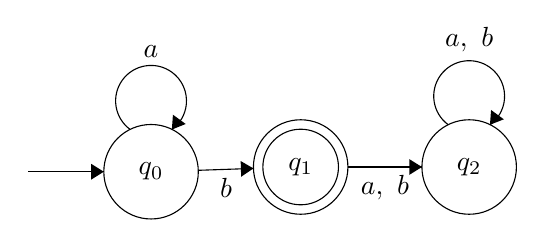
\begin{tikzpicture}[scale=0.2]
      \tikzstyle{every node}+=[inner sep=0pt]
      \draw [black] (15.1,-29.5) circle (3);
      \draw (15.1,-29.5) node {$q_0$};
      \draw [black] (24.6,-29.2) circle (3);
      \draw (24.6,-29.2) node {$q_1$};
      \draw [black] (24.6,-29.2) circle (2.4);
      \draw [black] (35.3,-29.2) circle (3);
      \draw (35.3,-29.2) node {$q_2$};
      \draw [black] (13.777,-26.82) arc (234:-54:2.25);
      \draw (15.1,-22.25) node [above] {$a$};
      \fill [black] (16.42,-26.82) -- (17.3,-26.47) -- (16.49,-25.88);
      \draw [black] (18.1,-29.41) -- (21.6,-29.29);
      \fill [black] (21.6,-29.29) -- (20.79,-28.82) -- (20.82,-29.82);
      \draw (19.87,-29.88) node [below] {$b$};
      \draw [black] (27.6,-29.2) -- (32.3,-29.2);
      \fill [black] (32.3,-29.2) -- (31.5,-28.7) -- (31.5,-29.7);
      \draw (29.95,-29.7) node [below] {$a,\mbox{ }b$};
      \draw [black] (33.977,-26.52) arc (234:-54:2.25);
      \draw (35.3,-21.95) node [above] {$a,\mbox{ }b$};
      \fill [black] (36.62,-26.52) -- (37.5,-26.17) -- (36.69,-25.58);
      \draw [black] (7.3,-29.5) -- (12.1,-29.5);
      \fill [black] (12.1,-29.5) -- (11.3,-29) -- (11.3,-30);
    \end{tikzpicture}
  \end{center}
  A machine only accepts \textbf{one} language. If it accept no strings, it
  recognizes the langauge \o. \\
  A palindrome is a string whose reversal is identical to the string.

  \subsection{Contex-Free Languages and Grammars}\noindent
  \begin{itemize}[noitemsep]
    \item A \textbf{regular expression} is a way of describing a regular
          language.
    \item A grammar gives the rules for expressing a language.
    \item A \textbf{context-free} language can be described by a
          \textbf{context-free grammar}.
    \item Theorem: A language is context-free if and only if some
          (nondeterministic) pushdown automaton recognizes it.
    \item A CFG is \textbf{ambiguos} if some string $w \in L(G)$ has at least
          two different leftmost derivations.
    \item Some context-free languages habe only ambiguous grammars.
  \end{itemize}
  Example: Designe a CFG for $L(G) = \{ww^R : w \in \{a, b\}^*\}$ \\
  \begin{align*}
    S & \rightarrow aSa     \\
    S & \rightarrow bSb     \\
    S & \rightarrow \lambda \\
    S & \rightarrow a|b
  \end{align*}

  \subsection{Turning Machines}\noindent
  A turing machine:
  \begin{itemize}[noitemsep]
    \item Reads input from tape, one character at a time.
    \item Changes state based on input.
    \item Outputs ``accept'' or ``reject'' when input ends.
  \end{itemize}
  In each step, a Turing machine \textbf{reads a symbol, writes a symbol, and
  moves left or right.} A turing machine cannot move left past the start of a
  tape, rather, it stays in place. \\
  A Turing machine has an accept stte and and a reject state. If it reaches one
  of these states, it outputs accept or rejects and stops reading input. An
  infinate loop means ``reject.'' \\

  \section{Limitations of Computational Models}\noindent
  \begin{itemize}[noitemsep]
    \item The language consisting of all Turing Machines encodings is an
          infinate set.
    \item Not all languages are recognizeable by a Turing Machine.
    \item Infinte sets come in different sizes.
  \end{itemize}

  \subsection{Countable vs. Uncountable Sets}\noindent
  \begin{itemize}[noitemsep]
    \item An infinite set $S$ is \textbf{countable} if and only if ther exists a
          bijective function $f: S \rightarrow Z^+$. $f$ maps each element of
          $S$ to exactly one element of $Z^+$ and every element of $Z^+$ is
          mapped by some element of $S$, under $f$.
    \item All infinite countable sets are the same size, the same size as $Z^+$.
    \item All finite sets are countable.
    \item \textbf{All subsets of countable sets are countable.}
  \end{itemize}

  \subsection{Enumerators}\noindent
  \begin{itemize}[noitemsep]
    \item An enumerator for a langage $S$ is a Turing Machine that generates
          all the strings in $S$ one by one. Each string is generated in finite
          time.
    \item \textbf{A set is countable if we can find an enumeration procedure for
          the set.}
    \item Theorem: The set of all Turing Machines is countable.
  \end{itemize}

  \subsection{Languages}\noindent
  \begin{itemize}[noitemsep]
    \item There are some languages not accepted by Turing Machines.
    \item These languages cannout be described by algorithms.
    \item A languages is called \textbf{Turing recognizable} if some Turing
          Machine recognizes it (aka accepts it).
    \item A language is called \textbf{Turing decidable} if some Turing machine
          decides it.
    \item Not all languages are recognizeable by a turing machine.
  \end{itemize}

  \section{Decision Problems}\noindent
  \begin{itemize}[noitemsep]
    \item \textbf{Decision problems} are problems with a YES or NO answer.
    \item A language is \textbf{Turing-decidable} if some Turing Machine decides
          it.
    \item The Turing Machine always halts.
    \item Theorem: The membersip problem is undecidable. There is no Turing
          Machine that can decide whether $M$ accepts $w$ for all $M$ and $w$.
    \item Theorem: The halting probelm is undecidable. There is no Turing
          machine that can determine whether $M$ halts on input for $w$ for all
          $M$ and $w$ (Proved in Turing's 1936 paper).
  \end{itemize}

  \section{P and NP}\noindent
  $$P \subseteq NP$$
  \begin{itemize}[noitemsep]
    \item Every language that can be decided by a deterministic Turing
          Machine in polynomial time can be decided by a nondeterministic
          Turing Machine in polynomial time.
    \item Every deterministic Turing Machine is a nondeterministic Turing
          Machine.
    \item Is $P = NP$? We don't know.
    \item Does the satisfiability problem have a polynomial time deterministic
          algorithm? We don't know.
    \item Cook's Theorem: The satisfiability problem is $NP$-complete.
  \end{itemize}

\end{multicols}

\end{document}
